\documentclass[11pt,letterpaper,titlepage]{article}

%================== Document nomenclature
\newcommand{\DOCSUBJT}{White Paper: }   %Put document subject here
\newcommand{\DOCTITLE}{                      %Put document title here
	Piecewise Linear Shape Functions on Polygon type cells
}       
\newcommand{\DOCDATE} {June, 2019}         %Put document date here
\newcommand{\DOCREV}  {Rev 1.00}             %Put revision number here

%================== Misc Settings
\usepackage{fancyhdr}
\usepackage[left=0.75in, right=0.75in, bottom=1.0in]{geometry}
\usepackage{lastpage}
\usepackage{titleref}
\usepackage{booktabs}
\usepackage{appendix}

\appendixtitleon
\appendixtitletocon

\makeatletter

%================== List of figures and tables mods
\usepackage{tocloft}
\usepackage[labelfont=bf]{caption}
\usepackage[linesnumbered,lined,boxruled,algosection,commentsnumbered]{algorithm2e}

\renewcommand{\cftfigpresnum}{Figure\ }
\renewcommand{\cfttabpresnum}{Table\ }

\newlength{\mylenf}
\settowidth{\mylenf}{\cftfigpresnum}
\setlength{\cftfignumwidth}{\dimexpr\mylenf+1.5em}
\setlength{\cfttabnumwidth}{\dimexpr\mylenf+1.5em}



%=================== Graphics
\usepackage{graphicx}
\usepackage[breakwords]{truncate}
\usepackage{float}
\usepackage{array}
\usepackage{amsmath}
\usepackage{mdframed}
\usepackage{fancyvrb}
\usepackage{float}
\usepackage{cancel}
\usepackage{amssymb}
\graphicspath{ {images/} }
\usepackage[usenames,dvipsnames,svgnames,table]{xcolor}
\usepackage[defaultlines=2,all]{nowidow}
\usepackage{listings}
\usepackage{color}
\definecolor{Brown}{cmyk}{0,0.81,1,0.60}
\definecolor{OliveGreen}{cmyk}{0.64,0,0.95,0.40}
\definecolor{CadetBlue}{cmyk}{0.62,0.57,0.23,0}
\usepackage{pdflscape}
\usepackage{relsize}
\usepackage{verbatim}
\usepackage{tabto}
\usepackage{upgreek}
\usepackage{enumitem}

\newcommand{\beq}{\begin{equation*}
\begin{aligned}}
\newcommand{\eeq}{\end{aligned}
\end{equation*}}

\newcommand{\beqn}{\begin{equation}
	\begin{aligned}}
\newcommand{\eeqn}{\end{aligned}
	\end{equation}}

%=================== Settings
\renewcommand{\baselinestretch}{1.2}
\definecolor{gray}{rgb}{0.4 0.4 0.4}
\newcommand{\stimes}{{\times}}
\setlength\parindent{0pt}

\newcommand{\xmltag}[1]{\textcolor{blue}{ \texttt{#1}} }
\newcommand{\xmloption}[1]{\textcolor{ao(english)}{ \texttt{#1}} }

%================== Code syntax highlighting
\lstset{language=C++,frame=ltrb,framesep=2pt,basicstyle=\linespread{0.8} \small,
	keywordstyle=\ttfamily\color{OliveGreen},
	identifierstyle=\ttfamily\color{CadetBlue}\bfseries,
	commentstyle=\color{Brown},
	stringstyle=\ttfamily,
	showstringspaces=true,
	tabsize=2,}
	
%=================== Big cdot
\newcommand*\bigcdot{\mathpalette\bigcdot@{.5}}
\newcommand*\bigcdot@[2]{\mathbin{\vcenter{\hbox{\scalebox{#2}{$\m@th#1\bullet$}}}}}

\begin{document}

\begin{titlepage}
	\pagestyle{fancy}
	\vspace*{1.0cm}
	\centering
	\vspace{1cm}
	\vspace{.25cm}
	{\Large\bfseries  \DOCSUBJT \par} 
	{\Large\bfseries \DOCTITLE  \par}
	\vspace{1cm}
	{\Large \DOCDATE \par}
	\vspace{1.0cm}
	{\Large Jan Vermaak \par}
	{\Large \DOCREV \par}

\end{titlepage}	


\pagestyle{fancy}
\rfoot{Page \thepage \ of \pageref{LastPage}}
\cfoot{}
\lfoot{\truncate{14cm}{\DOCTITLE}}
\rhead{}
\chead{\currentname}
\lhead{}
\renewcommand{\footrulewidth}{0.4pt}

\begin{comment}
\tableofcontents
\addtocontents{toc}{~\hfill\textbf{Page}\par}

\listoffigures
\listoftables

\end{comment}
\chead{Contents}	

%#########################################################################
\newpage
\chead{Triangle shape functions}
\section{Introduction - Piecewise linear shape functions on a 2D triangle}
For a two dimensional simulation using triangular elements we seek to map a triangle in cartesian space to a reference triangle in natural coordinates. We do this because we can develop a method to perform integration or differentation for the reference triangle that can be mapped to a triangle of any shape and location. An example of the two triangles in different coordinate space is shown in Figure \ref{fig:twodreferenceelement}.

\begin{figure}[H]
\centering
\includegraphics[width=0.8\linewidth]{Figures/TwoD_ReferenceElement}
\caption{Mapping of a 2D triangle to a reference triangle in natural coordinates.}
\label{fig:twodreferenceelement}
\end{figure}

The linear basis functions for the reference triangle are

\beq 
N_0(\xi,\eta) &= 1 - \xi - \eta \\
N_1(\xi,\eta) &= \xi \\
N_2(\xi,\eta) &= \eta. \\
\eeq 
From these functions we can interpolate the point $(x,y)$ with the following

\beq 
x &= N_0 x_0 + N_1 x_1 + N_2 x_2 \\
y &= N_0 y_0 + N_1 y_1 + N_2 y_2 \\
\eeq 
We can now express $x$ and $y$ as functions of $\xi$ and $\eta$ by substituting the expressions for $N_0$, $N_1$ and $N_2$ into the expressions for $x$ and $y$

\beq 
x &= (1-\xi-\eta)x_0 + (\xi)x_1 + (\eta)x_2 \\
&= x_0 -\xi x_0 -\eta x_0 +\xi x_1 +\eta x_2 \\
&= x_0 +(x_1 - x_0)\xi + (x_2 - x_0)\eta
\eeq 
and
\beq 
y &= (1-\xi-\eta)y_0 + (\xi)y_1 + (\eta)y_2 \\
&= y_0 -\xi y_0 -\eta y_0 +\xi y_1 +\eta y_2 \\
&= y_0 +(y_1 - y_0)\xi + (y_2 - y_0)\eta
\eeq 
\newline
In terms of the vectors from vertex $0$ to the other two vertices (refer to Figure \ref{fig:twodreferenceelement}) we can write this as

\beqn \label{eq:x2Dnat}
x = x_0 + \text{v}_{01x} \xi +\text{v}_{02x} \eta
\eeqn 
\beqn \label{eq:y2Dnat}
y = y_0 + \text{v}_{01y} \xi +\text{v}_{02y} \eta
\eeqn 
\newline
which is in the form of a linear transformation and from which we can determine the very important Jacobian matrix

\begingroup
\renewcommand*{\arraystretch}{1.5}
\beqn \label{eq:jacobiantriangle} 
\mathbf{J }= 
\begin{bmatrix}
\dfrac{dx}{d\xi}     & \dfrac{dx}{d\eta} \\
\dfrac{dy}{d\xi}     & \dfrac{dy}{d\eta} \\
\end{bmatrix}=
\begin{bmatrix}
\text{v}_{01x}  & \text{v}_{02x}  \\
\text{v}_{01y}  & \text{v}_{02y}  \\
\end{bmatrix}
=
\begin{bmatrix}
(x_1 - x_0) & (x_2 - x_0)  \\
(y_1 - y_0)  & (y_2 - y_0) \\
\end{bmatrix}.
\eeqn
\endgroup
\newline
The first application of the Jacobian will be for the integration of the trial or basis function in the finite element method. For simplicity let us consider the integration of a function over $x$ and $y$ which can be transformed to an integration of the linear transformation of function f, i.e. function g, over $\xi$ and $\eta$ using fundamental linear algebra. This integration is then

\beq 
\int \int f(x,y) .dx.dy = \int \int g (\xi,\eta).|J|.d\xi.d\eta
\eeq 
\newline
where $|J|$ is the determinant of the Jacobian. This integration can then easily be done either analytically or by using a quadrature rule. For the reference triangle this can easily be done using the method of undetermined coefficients as detailed in appendix \ref{appendix:trianglequadrature}.
\newline
\newline 
We need to define one more item that is related to the finite element method and that is the derivative of the basis functions, $\nabla N_i(\xi,\eta)$, which can be developed by noting that

\beq 
\frac{\partial N_i}{\partial \xi} = 
\frac{\partial N_i}{\partial x}\cdot \frac{\partial x}{\partial \xi} \ + \ 
\frac{\partial N_i}{\partial y}\cdot  \frac{\partial y}{\partial \xi}
\eeq 
\beq 
\frac{\partial N_i}{\partial \eta} = 
\frac{\partial N_i}{\partial x}\cdot \frac{\partial x}{\partial \eta} \ + \ 
\frac{\partial N_i}{\partial y}\cdot  \frac{\partial y}{\partial \eta}
\eeq 
\newline
which can be written as

\begingroup
\renewcommand*{\arraystretch}{1.5}
\beq
\begin{bmatrix}
\dfrac{\partial N_i}{\partial \xi} \\
\dfrac{\partial N_i}{\partial \eta}
\end{bmatrix}
&=
\begin{bmatrix}
\dfrac{\partial x}{\partial \xi}   &\dfrac{\partial y}{\partial \xi} \\
\dfrac{\partial x}{\partial \eta}   &\dfrac{\partial y}{\partial \eta} \\
\end{bmatrix}
\begin{bmatrix}
\dfrac{\partial N_i}{\partial x} \\
\dfrac{\partial N_i}{\partial y}
\end{bmatrix} \\
\therefore 
\begin{bmatrix}
\dfrac{\partial N_i}{\partial \xi} \\
\dfrac{\partial N_i}{\partial \eta}
\end{bmatrix}
&= \mathbf{J}^T 
\begin{bmatrix}
\dfrac{\partial N_i}{\partial x} \\
\dfrac{\partial N_i}{\partial y}
\end{bmatrix}.
\eeq 
\endgroup

Now we can invert $\mathbf{J}^T$ to get

\begingroup
\renewcommand*{\arraystretch}{1.5}
\beqn \label{eq:derivativeNtriangle}
\begin{bmatrix}
\dfrac{\partial N_i}{\partial x} \\
\dfrac{\partial N_i}{\partial y}
\end{bmatrix}
&=
(\mathbf{J}^T)^{-1}
\begin{bmatrix}
\dfrac{\partial N_i}{\partial \xi} \\
\dfrac{\partial N_i}{\partial \eta}
\end{bmatrix}
\eeqn 
\endgroup

and since the inverse of a $2\stimes 2$ matrix is given by

\beq 
\begin{bmatrix}
a & b\\
c & d
\end{bmatrix}^{-1}
=\frac{1}{ad-bc} 
\begin{bmatrix}
d & -b\\
-c & a
\end{bmatrix}
\eeq 

we have

\begingroup
\renewcommand*{\arraystretch}{1.5}
\beqn \label{eq:jacobianinversetriangle}
(\mathbf{J}^T)^{-1} =
\begin{bmatrix}
\dfrac{\partial x}{\partial \xi}   &\dfrac{\partial y}{\partial \xi} \\
\dfrac{\partial x}{\partial \eta}   &\dfrac{\partial y}{\partial \eta} \\
\end{bmatrix}^{-1}
&=
\frac{1}{|J|}
\begin{bmatrix}
\dfrac{\partial y}{\partial \eta}   & -\dfrac{\partial y}{\partial \xi} \\
-\dfrac{\partial x}{\partial \eta}  & \dfrac{\partial x}{\partial \xi} 
\end{bmatrix}
\eeqn
\endgroup





\newpage 
\chead{Piecewise linear shape functions on a 2D polygon}
\section{Piecewise linear shape functions on a 2D polygon}
The development of the methodology as applied to a 2D triangle has direct application when applied to a polygon since a polygon most likely presents more complexity than classical reference elements like quadrilaterals and therefore using triangles as grp_subsets of polygons overcomes this complexity. The use of subset triangles for the representation of a polygon was presented by Bailey \& Adams in \cite{BaileyAdamsPWLPolygons} the same authors which subsequently studied bi-linear basis functions \cite{BaileyAdamsPWBLPolygons}. From the latter paper it is this author's judgement that bi-linear basis functions offer little benefit over their linear counterparts and we will therefore pursue the linear methods presented in \cite{BaileyAdamsPWLPolygons}. The basis functions for each vertex of a polygon are of the form

\beqn 
P_i(x,y) = N_i(x,y) + \beta_i N_c(x,y)
\eeqn 
\newline
where the functions $N_i$ and $N_c$ are the standard linear functions defined on triangles. The subscripts $i$ and $c$ refer to the vertices $i$ and center of the polygon, respectively. The $\beta_i$ value is a weighting constant defined such that 

\beqn 
\begin{bmatrix}
x \\ y
\end{bmatrix}_{c}
= \sum_{s=0}^{N_{s}} \beta_s 
\begin{bmatrix}
x \\ y
\end{bmatrix}_{s,avg}.
\eeqn
\newline
Naturally it follows that $\beta_s = \dfrac{1}{N_{s}}$ where $N_s$ is the amount of sides. $[x \ y]_{s,avg}$ is the average coordinate of the two vertices of a side. An example basis function is shown in Figure \ref{fig:twodpolygon}. It should be noted that a single basis function now requires integration on each of the sub-triangles of the polygon instead of just a single one.

\begin{figure}[H]
\centering
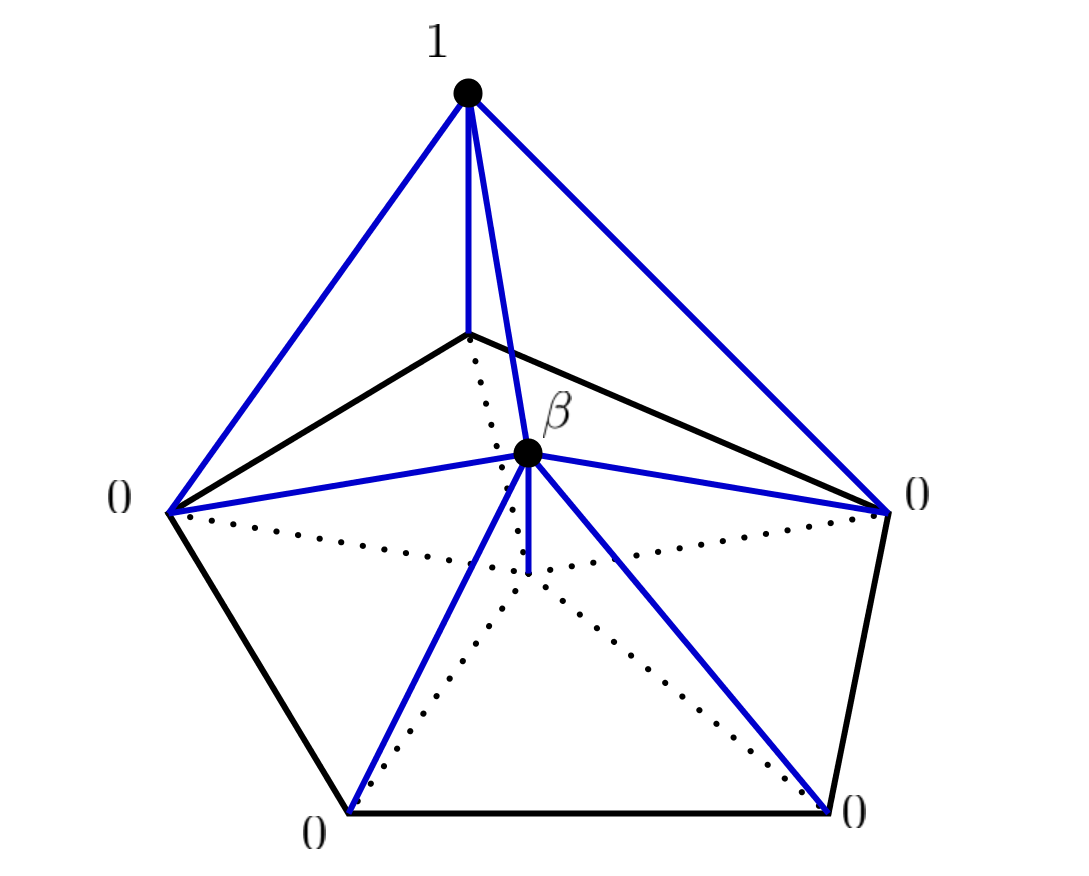
\includegraphics[width=0.5\linewidth]{Figures/TwoD_Polygon}
\caption{Basis function on a 2D polygon.}
\label{fig:twodpolygon}
\end{figure}


It is hard to visualize that this approach leads to an equivalent representation but with a few tests one can establish that this is equivalent. Some aspects of the paper presenting this method \cite{BaileyAdamsPWLPolygons} that are not intuitive is the explanation that integration is now over all sides. Also, the paper does not explicitly state that the cell centroid never features as an unknown in the solution. The customary assembly of the matrix in triangle or quadrilateral based meshes is to assemble cell-by-cell with an inner loop over the DOF of the cell. This approach is essentially the same but the paper states that integration is per side without saying that each DOF (except the cell center) of each side is also an inner loop of this integration. 
\newline
\newline
The method is versatile enough to applied to triangles and quadrilaterals where examples of the shape functions are shown in Figure

\begin{figure}[H]
\centering
\includegraphics[width=1.0\linewidth]{Figures/TwoD_PolygonTriQuad}
\caption{Basis functions on a triangle and on a quadrilateral.}
\label{fig:twodpolygontriquad}
\end{figure}




\newpage 
\chead{Volume Integrals}
\section{Volume Integrals}
\xmltag{IntV\_gradShapeI\_gradShapeJ[i][j]}

\xmltag{IntV\_shapeI\_gradshapeJ[i][j]}

\xmltag{IntV\_shapeI\_shapeJ[i][j]}

\xmltag{IntV\_shapeI[i]}

\vspace{0.5cm}
The finite element method requires the integration of the shape functions over the volume and surface of the cell. These integrations can easily be made analytically but for the purpose of being easy to follow we will revert to integration using a Gaussian quadrature. Let us discuss the assembly of the volume integrals, which for 2D polygons are essentially integrals over area multiplied by a unitary height. Before we do so we have to understand the assembly of the integrals in a triangle-by-triangle fashion. Volume integrals therefore take the form

\beqn 
\int_V P_i P_j .dV &= 
\int_V \biggr[
N_i + \beta_i N_c
\biggr]
 \biggr[
N_j + \beta_j N_c
\biggr].dV \\
&=\sum_{tris} \int_{V_{tri}}  \biggr[
N_i + \beta_i N_c
\biggr]
 \biggr[
N_j + \beta_j N_c
\biggr].dV_{tri}
\eeqn
\newline
Now let 

\beq
F(x,y) =  \biggr[
N_i + \beta_i N_c
\biggr]
 \biggr[
N_j + \beta_j N_c
\biggr]
\eeq 
\newline 
With this definition we now have the more general form of a function evaluated triangle-by-triangle which is represented by

\beqn 
\int_V P_i P_j .dV = \int_V F(x,y).dV 
= \sum)_{tris} \int_{V_{tri}} F(x,y).dV_{tri}
\eeqn 
\newline
for which we can first transform the integral over cartesian coordinate version of a triangle ($V_{tri}$) to an integral over the natural coordinates version ($V_\tau$) as

\beqn 
\int_{V_{tri}} F(x,y).dV_{tri} = \int_{V_{\tau}} F(\xi,\eta).dV_\tau.|J|_{tri}
\eeqn 
\newline
and then apply an appropriate Gaussian quadtrature for the volume integral

\beqn 
\int_{V_{\tau}} F(\xi,\eta).dV_\tau.|J|_{tri} = 
\sum_q^Q F((\xi,\eta)_q).w_q.|J|_{tri}
\eeqn 
\newline
where $w_q$ is the quadrature weight associated with the quadtrature abscissa $q$, a unique comination of $\xi$ and $\eta$. These weights and abscissae are tabulated in Appendix A.




\vspace{0.5cm}
\chead{Surface Integrals}
\section{Surface Integrals}
\xmltag{IntS\_shapeI\_shapeJ[f][i][j]}

\xmltag{IntS\_shapeI[f][i]}

\xmltag{IntS\_shapeI\_gradshapeJ[f][i][j]}

\vspace{0.5cm}
The same form of the volume integrals can be encountered on surfaces of the cell (in this case an edge). To this end we can use the convention depicted in Figure \ref{fig:twodedgetriangle}. With the first leg of the triangle defined along $\xi$ the integral along the edge of the triangle is always an integral from 0 to 1 along the natural coordinates.

\beq 
v_0 &= \text{Edge vertex 0}\\
v_1 &= \text{Edge vertex 1}\\
v_2 &= \text{Cell center}
\eeq 

\begin{figure}[H]
\centering
\includegraphics[width=0.9\linewidth]{Figures/TwoD_EdgeTriangle}
\caption{Orientation of a triangle on a cell.}
\label{fig:twodedgetriangle}
\end{figure}

Surface integrals can now take the simple form of the volume integrals without any special treatment

\beqn 
\int_{side} F(x,y).dA_{side} = \sum_q^Q F(\xi_q,\eta).w_q.|J|_{surf}
\eeqn 

The determinant on the surface, $|J|_{surf}$, is simply the length of the edge in cartesian coordinates. Quadrature weights and abscissae for integration are depicted in Appendix B.


\chead{Coding implementation}
\section{Coding implementation}
\subsection{5.1 Constructor \xmltag{00\_constrdestr.cc}}
In the constructor we receive the basic cell information (i.e. information about vertices and edges), a reference to the grid (holding actual vertex values) and the discretization method (holding quadrature information).
\begin{lstlisting}[language=c++]
content...
\end{lstlisting}
\begin{lstlisting}[language=c++]
PolygonFEView(chi_mesh::CellPolygon* poly_cell,
              chi_mesh::MeshContinuum* grid,
              SpatialDiscretization_PWL *discretization)
\end{lstlisting}

\begin{itemize}
\item We immediately make reference copies of the quadrature sets and obtain the cell center.
\item We then construct each triangle of the polygon by looping over the edges of the cell
\begin{itemize}
\item For each edge we instantiate a new data structure, \xmltag{FEside\_data2d}, which holds the triangle data.
\item For each edge we form the $v_{01}$ leg of the triangle by the cell edge. And the $v_{02}$ leg as the edge from the first vertex of the edge to the cell centre.
\item Since the determinant of the area is easy to compute we do it here.
\item Since the length of the $v_{01}$ leg is unity in natural coordinates, the edge determinant (more generally surface determinant) is simply the length ($L_2$-norm) of the $v_{01}$ leg.
\item We then compute the Jacobian, Jacobian inverse and the Jacobian-transpose inverse
\end{itemize}
\item In order to determine if a given cell DOF is associated with vertex 0 or vertex 1 of a given triangle we have to develop a node-to-side mapping.
\item Lastly a useful mapping is developed where, given a side and side DOF index, we can obtain the associated cell DOF. This is useful when assembling matrices.
\end{itemize}



\vspace{0.5cm}
\subsection{Precomputing the integrals}
The precompute function, also called the phase of ``computing cell matrices", is a function which pre-computes the quadrature rule based integrals. For its first phase it computes the values of the different shape functions on every triangle and every quadrature point. To this end the code relies on the following functions:

\vspace{0.5cm}
\textbf{Defined in } \xmltag{02\_compcellmat.cc}
\begin{lstlisting}[language=c++]
double PreShape(int s, int i, int qpoint_index, bool on_surface = false);
double PreGradShape_x(int s, int i, int qpoint_index);
double PreGradShape_y(int s, int i, int qpoint_index);
\end{lstlisting}

These functions use the developed \xmltag{FEside\_data2d} data structure to evaluate the side shape functions from the reference triangle function.
\newline
\newline
As an example consider \xmltag{PreGradShape\_x}:
\newline 
\begin{lstlisting}[language=c++]
double PolygonFEView::PreGradShape_x(int s, int i, int qpoint_index)
{
  int index = node_to_side_map[i][s];
  double value = 0;
  if (index==0)
  {

    value = sides[s]->JTinv.GetIJ(0,0)*-1.0 +
            sides[s]->JTinv.GetIJ(0,1)*-1.0;
  }
  if (index==1)
  {

    value = sides[s]->JTinv.GetIJ(0,0)*1.0 +
            sides[s]->JTinv.GetIJ(0,1)*0.0;
  }

  value += beta*(sides[s]->JTinv.GetIJ(0,0)*0.0 +
                 sides[s]->JTinv.GetIJ(0,1)*1.0);


  return value;
}
\end{lstlisting}

This trail culminates in the following portion of the \xmltag{PreCompute} phase:
\begin{lstlisting}[language=c++]
for (int s=0; s<num_of_subtris; s++)
{
	for (int i=0; i<dofs; i++)
	{
	  FEqp_data2d* pernode_data = new FEqp_data2d;
	  for (int q=0; q<vol_quadrature->qpoints.size(); q++)
	  {
	    pernode_data->shape_qp.push_back(PreShape(s, i, q));
	    pernode_data->gradshapex_qp.push_back(PreGradShape_x(s, i, q));
	    pernode_data->gradshapey_qp.push_back(PreGradShape_y(s, i, q));
	  }//for qp
	
	  for (int q=0; q<surf_quadrature->abscissae.size(); q++)
	  {
	    //printf("%g\n",PreShape(s,i,q,ON_SURFACE));
	    pernode_data->shape_qp_surf.push_back(PreShape(s,i,q,ON_SURFACE));
	  }
	  sides[s]->qp_data.push_back(pernode_data);
	}//for dof
}//for side
\end{lstlisting}

With the values of the shape functions evaluated at the quadrature points the second phase of the \xmltag{PreCompute} function assembles the integrals as if we were assembling a matrix by using the quadrature points. It has many facets and a number of utility functions but should be intuitive to follow.


\vspace{0.5cm}
\chead{Using interpolation}
\section{Using interpolation}
Two utility functions are available for use by field function interpolators:

\vspace{0.5cm}
\textbf{Defined in } \xmltag{01\_xy\_shapefuncs.cc}
\begin{lstlisting}[language=c++]
double Shape_xy(int i, chi_mesh::Vector xyz);
chi_mesh::Vector GradShape_xy(int i, chi_mesh::Vector xyz);
\end{lstlisting}

These functions are used with cartesian coordinates and returns the values of the shape functions in the cartesian reference frames.






\newpage
\chead{Appendices}
\begin{appendices}
\renewcommand{\thefigure}{D\arabic{section}.\arabic{figure}}
\chead{Quadrature rule for integration of triangle space}
\section{Quadrature rule for integration of triangle space} \label{appendix:trianglequadrature}
We seek an integral of a function in triangle space $T_{sp}$ in the form

\beq 
\int \int_{T_{sp}} f(x,y).dx.dy = \sum_{i=0}^{N-1} w_i f(x_i,y_i).
\eeq 

Furthermore we know that in the finite element method with only linear shape functions we will at most have polynomials of degree 2 therefore we can devise a set of test functions

\beq 
&f(x,y) = 1    &&\int_{0}^1 \int_0^{1-y} 1.dx.dy = \frac{1}{2} = \sum_{i=0}^{N-1} w_i\\
&f(x,y) = x    &&\int_{0}^1 \int_0^{1-y} x.dx.dy = \frac{1}{6} = \sum_{i=0}^{N-1} w_i x_i\\
&f(x,y) = y    &&\int_{0}^1 \int_0^{1-y} y.dx.dy = \frac{1}{6} = \sum_{i=0}^{N-1} w_i y_i\\
&f(x,y) = xy  & &\int_{0}^1 \int_0^{1-y} xy.dx.dy = \frac{1}{24} = \sum_{i=0}^{N-1} w_i x_i y_i\\
&f(x,y) = x^2    &&\int_{0}^1 \int_0^{1-y} x^2.dx.dy = \frac{1}{12} = \sum_{i=0}^{N-1} w_i x_i^2\\
&f(x,y) = y^2    &&\int_{0}^1 \int_0^{1-y} y^2.dx.dy = \frac{1}{12} = \sum_{i=0}^{N-1} w_i y_i^2\\
\eeq 

With $N=3$ a symmetric solution is obtained with

\beq
w_i &= \frac{1}{6} \\
x_0,y_0 &= ( \frac{1}{6}, \frac{1}{6}) \\
x_1,y_1 &= ( \frac{4}{6}, \frac{1}{6}) \\
x_2,y_2 &= ( \frac{1}{6}, \frac{4}{6}) \\
\eeq 
which is not a unique solution.

\newpage 
\chead{Quadrature rule for integration of triangle edge}
\section{Quadrature rule for integration of triangle edge}
Along the edge of a triangle the integration reverts to a one dimensional integral

\beqn 
\int_S F(x,y) .dA \to \int_e F(x,y).ds = \int_{e} F(\xi,\eta).ds.|J| 
\eeqn 

In natural coordinates we will mostly deal with the following integral

\beqn 
\int_{0}^{1} F(\xi,\eta).d\xi &= \frac{1}{2} \int_{-1}^{+1} F(y,\eta).dy \\
&=\frac{1}{2} \sum_{q=0}^{1} w_q F(y_q,\eta)
\eeqn 
where $y=\frac{1}{2} \xi + \frac{1}{2}$ and for which the quadrature rule is 

\beq 
y_0 &=  +\frac{1}{\sqrt{3}} \quad \quad w_0 = 1\\
y_1 &=  -\frac{1}{\sqrt{3}} \quad \quad w_1 = 1
\eeq 
\newline
Now when translated back to natural coordinates in the form

\beq 
\int_{0}^{1} F(\xi,\eta).d\xi = \sum_{q=0}^1 w_q' F(\xi_q,\eta)
\eeq 

we get the quadrature rule

\beq 
\xi_0 &=  +\frac{1}{2\sqrt{3}} +\frac{1}{2}\quad \quad w_0 =\frac{1}{2}\\
\xi_1 &=  -\frac{1}{2\sqrt{3}}+\frac{1}{2} \quad \quad w_1 = \frac{1}{2}
\eeq 

\end{appendices}

\newpage
\chead{References}
\begin{thebibliography}{1}
    
    \bibitem{BaileyAdamsPWLPolygons}  Bailey T.S., Chang J.H., Adams M.L., {\em A Piecewise Linear Discontinous Finite Element spatial discretization of the transport equation in 2D Cylindrical Geometry}, 2009 International Conference on Advances in Mathematics, Computational Methods, and Reactor Physics, 2008.
    
     \bibitem{BaileyAdamsPWBLPolygons}  Bailey T.S., Warsa J.S., Chang J.H., Adams M.L., {\em A Piecewise Bi-linear Discontinous Finite Element spatial discretization of the S$_n$ transport equation}, International Conference on Mathematics and Computational Methods Applied to Nuclear Science and Engineering, 2011.
    
\end{thebibliography}





\end{document}